% Reading Wealth from Above -- 35-minute lab talk, October 2026
% Compile with XeLaTeX twice. All displayed figure dependencies are local.
% To show speaker notes: define \shownotes before inputting this file.
% Main deck has no automatic overlays or section-divider pages.
\documentclass[11pt,aspectratio=169]{beamer}
\usetheme[nosectionpages,noprogressbar,nouppercase]{marginal}
\usepackage{amsmath,amssymb,mathtools,tabularx,array,graphicx,pgfpages}
\usepackage{appendixnumberbeamer}
\ifdefined\shownotes\setbeameroption{show notes on second screen=right}\else\setbeameroption{hide notes}\fi
\setbeamertemplate{navigation symbols}{}
\setbeamersize{text margin left=8mm,text margin right=8mm}
\definecolor{mgBg}{HTML}{FFFFFF}
\definecolor{mgText}{HTML}{28323B}
\definecolor{mgMuted}{HTML}{56616B}
\setbeamercolor{normal text}{fg=mgText,bg=white}
\setbeamerfont{frametitle}{family=\sffamily,size=\large,series=\bfseries}
\setbeamerfont{title}{family=\sffamily,size=\LARGE,series=\bfseries}
\setbeamertemplate{frametitle}{\par\vspace{4mm}\insertframetitle\par\par\vspace{2mm}{\color{mgAccent}\rule{12mm}{1.1pt}}\par\vspace{1mm}}
\setbeamertemplate{footline}{\hbox to\paperwidth{\hspace{8mm}{\scriptsize\color{mgMuted}Nicol\'as Abbate\quad|\quad Vives Lab}\hfill{\scriptsize\color{mgMuted}\insertframenumber\,/\,\inserttotalframenumber}\hspace{8mm}}\par\vspace{3mm}}
\setlength{\parskip}{.25em}
\setbeamertemplate{itemize item}{\raisebox{.2ex}{\color{mgAccent}\tiny$\bullet$}}
\newcommand{\takeaway}[1]{\par{\color{mgAccent}\normalsize\bfseries #1\par}}
\newcommand{\source}[1]{\par{\scriptsize\color{mgMuted}#1\par}}
\newcommand{\pending}[2]{\begingroup\setlength{\fboxsep}{9pt}\color{mgRule}\fbox{\parbox[c][#2][c]{.88\linewidth}{\centering\color{mgMuted}\small #1\par\medskip\scriptsize Figure forthcoming}}\endgroup}
\newcommand{\resultslot}[2]{\IfFileExists{#1}{\includegraphics[width=\linewidth,height=3.7cm,keepaspectratio]{#1}}{\pending{#2}{3.4cm}}}
\newcommand{\resultslotwide}[2]{\begin{center}\IfFileExists{#1}{\includegraphics[width=.92\textwidth,height=3.7cm,keepaspectratio]{#1}}{\begin{minipage}{.88\textwidth}\pending{#2}{3.4cm}\end{minipage}}\end{center}}
\newcommand{\puzzletile}[1]{\IfFileExists{figures/puzzle/#1.png}{\includegraphics[width=2.5cm,height=1.6cm,keepaspectratio]{figures/puzzle/#1.png}}{\fcolorbox{mgRule}{white}{\parbox[c][1.4cm][c]{2.3cm}{\centering\scriptsize\color{mgMuted}Image forthcoming}}}}
\title{Reading Wealth from Space}
\author{Nicol\'as F. Abbate}
\date{Vives-i-Bastida Lab\quad October 2026}
\begin{document}
\begin{frame}[plain,noframenumbering]
\par\vspace{.6cm}
{\color{mgAccent}\rule{17mm}{1.4pt}}\par\bigskip
{\LARGE\bfseries Reading Wealth from Space\par}
\par\vspace{.45cm}
{\large A common index across places and years\par}
\par\vspace{1.0cm}
Nicol\'as F. Abbate\par
\small NYU\par\medskip
Vives-i-Bastida Lab\quad October 2026
\note{0:15. A measurement agenda motivated by economic panels. Target 35 minutes including the forthcoming simulation figures, leaving about 25 minutes for lab discussion.}
\end{frame}
\begin{frame}[label=s1]{Can imagery fill gaps between surveys?}

\begin{columns}[c]
\column{.53\textwidth}
\large Economic policy needs to know\par\medskip
\textbf{where people are poor}\par\medskip
and \textbf{where conditions are changing}.
\column{.43\textwidth}
\textcolor{mgAccent}{\textbf{A use already in practice}}\par\medskip
Togo's Novissi program used satellite wealth maps to select poor areas.\par\medskip
Phone data then helped select recipients within those areas.
\end{columns}
\par\vfill\source{Aiken et al. (2022); CEGA, AI-assisted cash transfers in Togo}

\note{1:00. Motivate the economic problem before the method. Satellite maps supported geographic targeting, not direct household identification. Source: https://cega.berkeley.edu/collection/ai-assisted-cash-transfers-togo/ . The World Bank Geospatial Poverty Portal provides a second example of institutional demand.}
\end{frame}

\begin{frame}[label=s2]{Good rankings; economic change remains difficult}

\large Can we learn a common economic index when labels\par
mean different things across places and years?
\par\vspace{.7cm}
\begin{columns}[T]
\column{.30\textwidth}\textcolor{mgAccent}{\Large 35 of 36}\par\medskip
Test cities with higher tract-level ranking accuracy than L2
\column{.30\textwidth}\textcolor{mgAccent}{\Large Common index}\par\medskip
Within-cell rankings + restrictions on stable pairs
\column{.32\textwidth}\textcolor{mgRed}{\Large Change: not yet}\par\medskip
Construction response does not deliver accurate tract-level changes
\end{columns}

\note{1:00. Preview findings now, following Shapiro. The 35/36 comparison is a comparison of fitted runs, with unequal total training budgets (750 versus 200 epochs), not a clean equal-compute loss ablation. Change result is after GB2 calibration. Source: run\_20260722 evaluation tables and NYC F\_construction\_scatter.pdf.}
\end{frame}

\begin{frame}[label=s3]{Four questions in one research agenda}

\begin{tabularx}{\textwidth}{@{}l X@{}}
\textcolor{mgAccent}{\textbf{Today}} & Learn from non-comparable labels\\[.5cm]
 & Test the framework in US cities\\[.6cm]
\textcolor{mgMuted}{\textbf{Next}} & Identify economic change between surveys\\[.5cm]
 & Establish when predicted outcomes support policy evaluation
\end{tabularx}
\par\vfill
\takeaway{The long-run goal is a credible economic panel from imagery.}

\note{0:30. Four connected research questions, not completion percentages or a promise of four papers. Global pretraining plus local survey calibration is the ambition; causal use requires additional validation.}
\end{frame}

\begin{frame}[label=s4]{What existing imagery models already deliver}

\begin{tabularx}{\textwidth}{@{}p{3.0cm} X@{}}
\textbf{Asset wealth} & Strong spatial predictions; recent models explicitly predict decadal change.\\[.5cm]
\textbf{Income growth} & Khachiyan et al. study microspatial economic growth.\\[.5cm]
\textbf{This project} & Learn an index under \emph{unknown cell-specific monotone transformations}, using rankings and stability.
\end{tabularx}
\par\vfill\source{Jean et al. (2016); Yeh et al. (2020); Khachiyan et al. (2022); Zheng et al. (2026)}

\note{0:45. Avoid claiming that nobody predicts change. Tempov reports decadal asset-wealth change R2 around .69 and .46 in Malawi and Mozambique. Source: https://arxiv.org/html/2604.23166v1 . Khachiyan et al.: https://doi.org/10.1257/aeri.20210422 . The contribution is a measurement framework, not merely applying AI to a new geography.}
\end{frame}

\begin{frame}[label=s5]{The US measurement setting}

\begin{columns}[T]
\column{.50\textwidth}
\textcolor{mgAccent}{\textbf{What the model sees}}\par\medskip
NAIP aerial imagery around building locations\par\medskip
224\,$\times$\,224 metre footprint in the saved run; 224\,$\times$\,224 pixels
\column{.44\textwidth}
\textcolor{mgAccent}{\textbf{What supervises it}}\par\medskip
ACS five-year estimates\par\medskip
A constructed wealth index at the \textbf{census-tract} level
\end{columns}
\par\vspace{.1cm}
\begin{center}
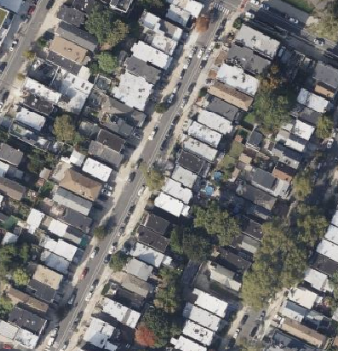
\includegraphics[width=.24\textwidth,height=1.7cm,keepaspectratio]{figures/image3.png}\hspace{.3cm}
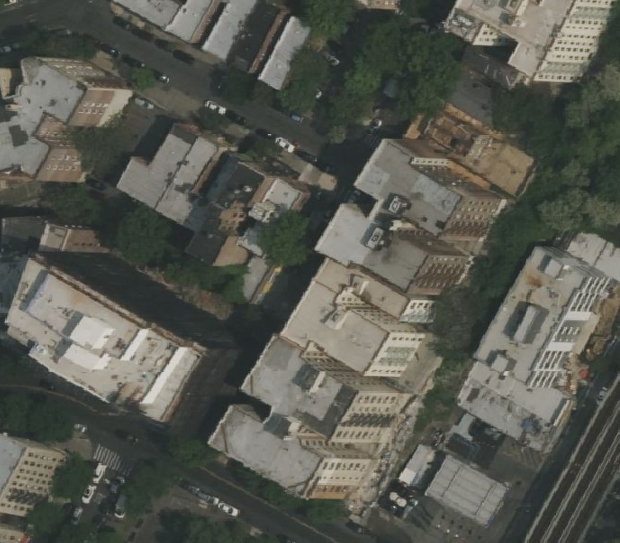
\includegraphics[width=.24\textwidth,height=1.7cm,keepaspectratio]{figures/image2.png}\hspace{.3cm}
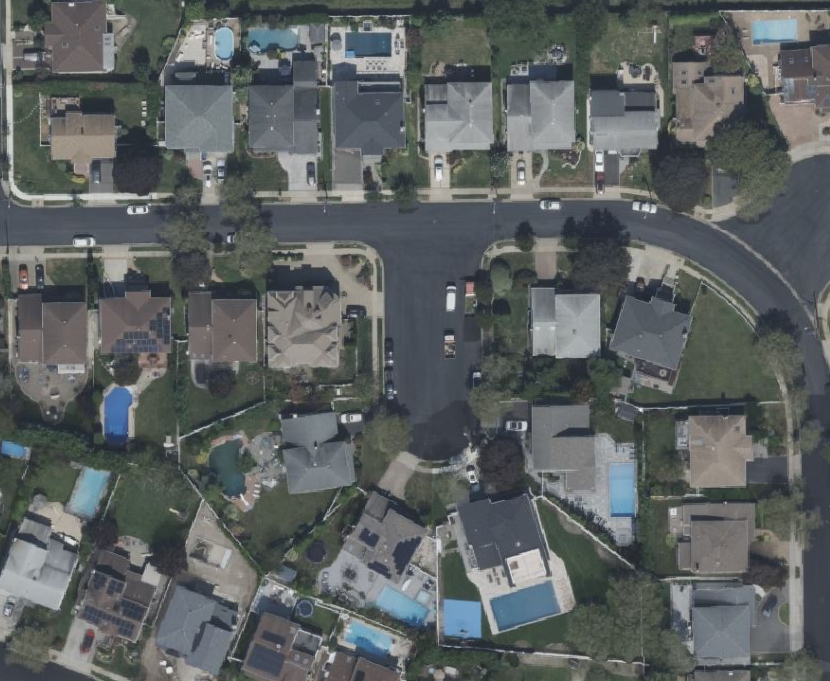
\includegraphics[width=.24\textwidth,height=1.7cm,keepaspectratio]{figures/image1.png}
\end{center}
\takeaway{Predictions at building locations; validation at the tract level.}

\note{1:00. Establish observation units early. Illustrative local imagery from the previous deck; these are not certified training crops. Logged tau is 112m, after snapping requested 100m; 224 pixels. Data sources: USDA NAIP, ACS, Microsoft US Building Footprints. Saved run log and debug\_batches/dump\_info.json support geometry. Avoid claiming household or building wealth is directly observed.}
\end{frame}

\begin{frame}[label=s6]{The label is a constructed wealth measure}

\[
W2_{it}=\underbrace{y^L_{it}\frac{1-(1+r_d)^{-N_{it}}}{r_d}}_{\text{human wealth}}
+\underbrace{\frac{y^K_{it}}{r_k}}_{\text{capitalized income}}
+\underbrace{\frac{A^H_{it}}{P_{it}}(1-m_{it}\ell_t)}_{\text{housing equity}}
\]
\par\vspace{.2cm}
\begin{itemize}
\item $y^L,y^K$: annual earnings and capital income per capita
\item $N$: expected remaining working years; $r_d=5\%$, $r_k=4.5\%$
\item $A^H/P$: owner housing value per capita; $m$: mortgaged-owner share; $\ell_t$: aggregate LTV input
\end{itemize}
\par\vfill\takeaway{An ACS-based proxy for occupant wealth, not a direct net-worth survey.}

\note{1:15. Formula checked against src/data/process\_acs.py annuity\_factor, equity\_pc and wealth\_from\_inputs. Ordinary annuity begins at period 1, not 0. Mortgage share m is required by code. Use r\_d for discount rate to avoid collision with the comparison-error precision rho. This describes the implemented index, not an independent validation of its economic construction. LTV source and potential aggregate/share interpretation are in backup.}
\end{frame}

\begin{frame}[label=s7]{Similar structures can carry different dollar labels}

\begin{center}
\begin{tabular}{rccc}
& Higher & Middle & Lower\\[4pt]
NYC & \puzzletile{nyc_rich} & \puzzletile{nyc_mid} & \puzzletile{nyc_poor}\\[6pt]
Chicago & \puzzletile{chi_rich} & \puzzletile{chi_mid} & \puzzletile{chi_poor}
\end{tabular}
\end{center}
\par\vfill\takeaway{The economic claim to test: a common ordering can survive local rescaling.}

\note{1:00. Six images will arrive tomorrow. Replace exact filenames in figures/puzzle; no invented labels or footprint overlays. Give each its actual tract/year label using the configurable labels in the preamble if desired. Similarity is illustrative, not evidence that A2 holds. Keep this slide to one minute; footprints can be discussed using a backup image if useful.}
\end{frame}

\begin{frame}[label=s8]{Image changes need not be economic changes}

\begin{center}
\begin{tabular}{ccc}
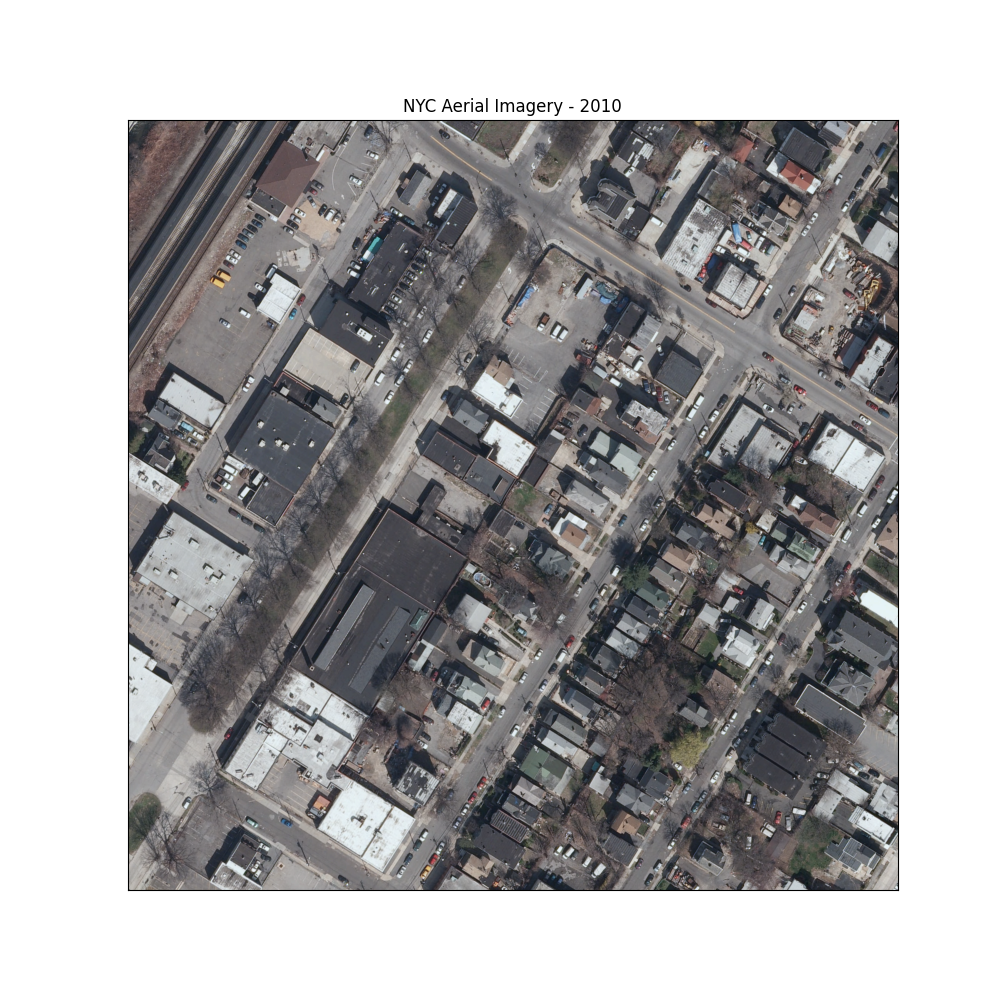
\includegraphics[width=.275\textwidth]{figures/nyc_years/nyc_2010.png}&
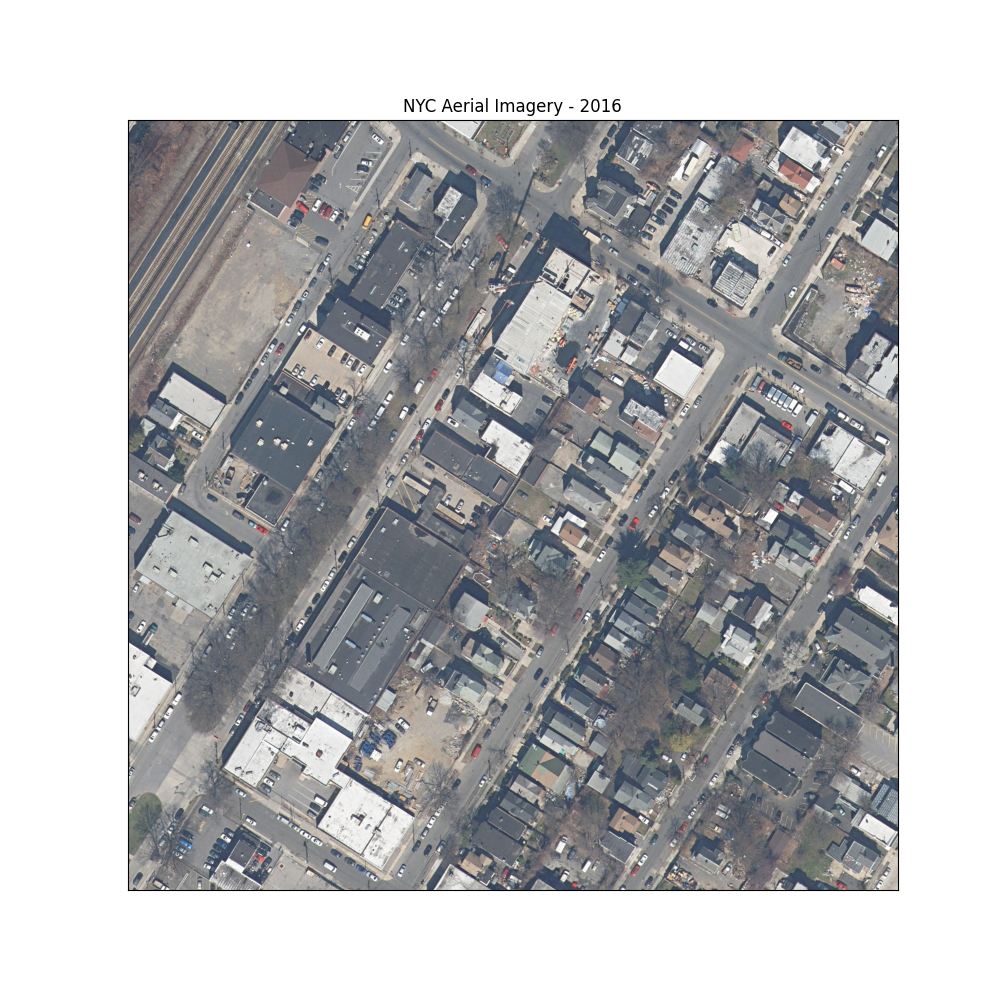
\includegraphics[width=.275\textwidth]{figures/nyc_years/nyc_2016.png}&
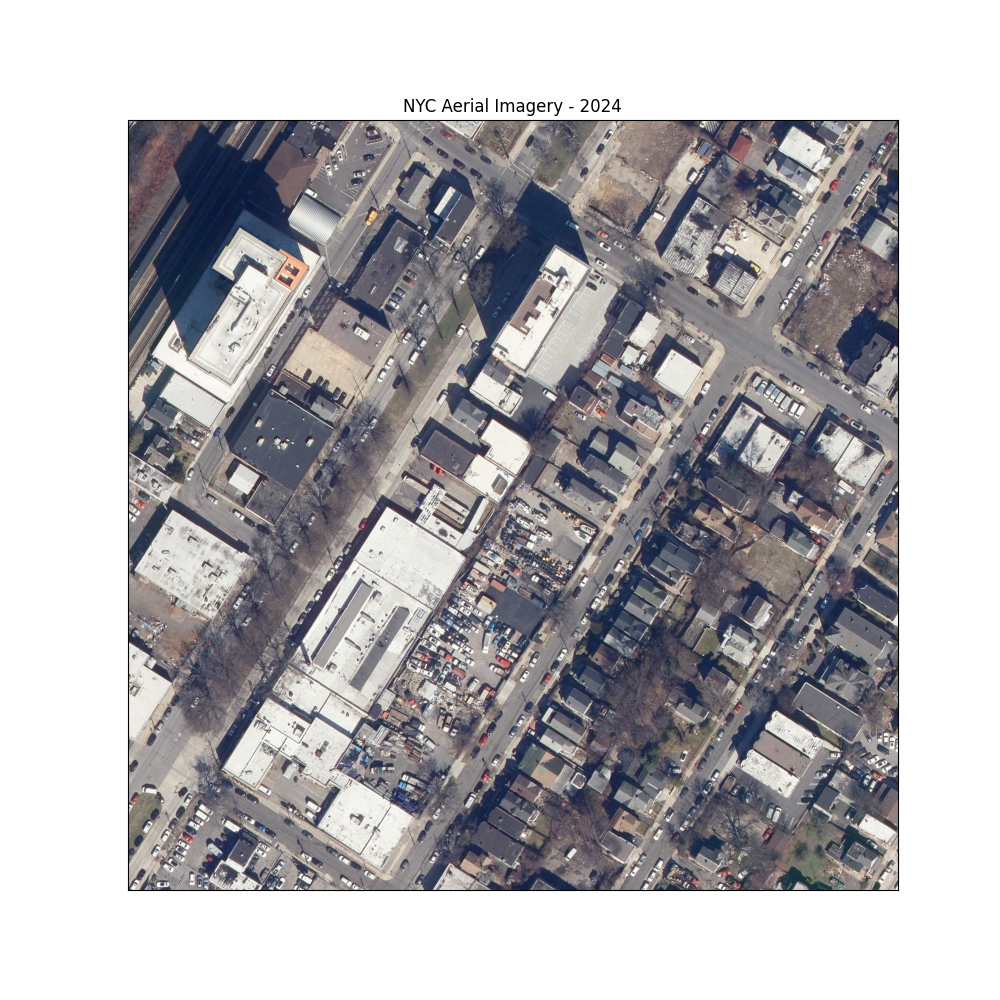
\includegraphics[width=.275\textwidth]{figures/nyc_years/nyc_2024.png}\\[6pt]
2010 & 2016 & 2024
\end{tabular}
\end{center}
\par\vfill
\takeaway{Acquisition conditions and physical development can both change the pixels.}

\note{0:45. Images copied from supplied NYC time-series location. Inspect structures and acquisition differences live; do not assert that the entire scene is physically unchanged. Label-scale variation and acquisition variation are distinct problems. Stability restrictions concern selected pairs, not every location.}
\end{frame}

\begin{frame}[label=s9]{A common index with a local measurement scale}

\[
\underbrace{W_{ict}}_{\text{observed label}}
=\underbrace{\psi_{ct}}_{\text{local scale}}\!\left(\underbrace{R_{ict}}_{\text{latent index}}\right),
\qquad R_{ict}=\underbrace{\textcolor{mgAccent}{f(X_{ict})}}_{\text{target}}+\varepsilon_{ict}
\]
\par\vspace{.5cm}
\begin{itemize}
\item A cell $(c,t)$ is one city and one date
\item $\psi_{ct}$ absorbs differences in level, spread and shape
\item Estimate the systematic index $f$ without estimating $\psi_{ct}$
\end{itemize}
\par\vfill\takeaway{The score targets $f(X)$, not a realized $R$ or a dollar conditional mean.}

\note{1:45. Define all notation explicitly. Moving an additive outcome error through an invertible psi is only a reparameterization; it does not imply latent mean zero or logistic differences. Those restrictions are additional. Model is not an empirical proof that all city differences are monetary rescalings. Pooled-level proposition and derivation in backup.}
\end{frame}

\begin{frame}[label=s10]{The central economic restriction is invariance}

\textcolor{mgAccent}{\textbf{A1. Monotonicity}}\par\medskip
$\psi_{ct}$ is strictly increasing within each city-year.
\par\vspace{.7cm}
\textcolor{mgAccent}{\textbf{A2. Invariance}}\par\medskip
The same function $f$ maps features into the index in every cell.
\par\vfill\takeaway{A2 rules out reversals in the economic meaning of feature bundles.}

\note{1:00. This is where the audience should interrogate the model. A pool or density is not guaranteed to mean the same thing everywhere. Shared function plus geographic cues can also reproduce city-specific behavior on disjoint supports. No claim of universal extrapolation. Units here are tract labels paired with local views.}
\end{frame}

\begin{frame}[label=s11]{Stable pairs add a second source of information}

\textcolor{mgAccent}{\textbf{A3. Regularity and valid pairs}}
\[
 f=g\circ\phi,\quad H=\phi(X),\qquad
 |g(h')-g(h)|\le L\|h'-h\|
\]
\[
 (x,x')\in\mathcal S:\quad\|\phi(x')-\phi(x)\|\le\delta
 \quad\Longrightarrow\quad |f(x')-f(x)|\le L\delta
\]
\begin{itemize}
\item Standardized representation; nonconstant index within cells
\item Theory: choose pairs without reference to the labels
\item Examples: footprint records or an independent image-change detector
\end{itemize}

\note{1:15. A3 restricts the true systematic score, not realized occupant wealth. No footprint change is an imperfect proxy, not a proof. L and delta are not observed; tightening the selection rule is intended to improve pair validity, not guaranteed to reduce latent delta. Occupant sorting and earnings can change without visible structure changes.}
\end{frame}

\begin{frame}[label=s12]{Within-cell comparisons eliminate the local scale}

\[
 y_{ij}=\mathbf1\{W_j>W_i\}=\mathbf1\{R_j>R_i\},
 \qquad \Delta_{ij}f=f(X_j)-f(X_i)
\]
\par\vspace{.3cm}
\textcolor{mgAccent}{\textbf{A4(c). Homogeneous logistic comparison errors}}
\[
 \Pr(y_{ij}=1\mid X_i,X_j,c,t)=\Lambda(\rho\Delta_{ij}f),
 \qquad \Lambda(z)=\frac{1}{1+e^{-z}}
\]
\par\vfill
\takeaway{Label order is observed; recovering score differences needs an error model.}
\smallskip\small Median-zero errors and cell-specific $\rho_{ct}$ are extensions.\hfill\hyperlink{errors}{\beamergotobutton{A4 variants}}

\note{1:15. Logistic is imposed on epsilon\_i minus epsilon\_j, not on individual residuals. Common rho fixes a common comparison-noise scale. Feature-dependent residual dispersion is excluded by this version. The weaker median-zero version requires a suitable strict crossing condition; results for it are not yet claimed.}
\end{frame}

\begin{frame}[label=s13]{The criterion combines ranking and stability}

\[
Q(s)=\underbrace{\mathbb E_{\mathcal C}\ell(\Delta_{ij}s,y_{ij})}_{Q_{\rm cross}(s)}
+\lambda\underbrace{\frac{S(s)}{V(s)}}_{\text{stability / within-cell spread}}
\]
\[
S(s)=\mathbb E_{\mathcal S}(s(x')-s(x))^2,
\qquad V(s)=\tfrac12\mathbb E_{\mathcal C}(\Delta_{ij}s)^2
\]
\begin{itemize}
\item $\ell(z,y)=\log(1+e^z)-yz$: pairwise logistic loss
\item Increasing relabelings preserve the comparisons
\item Dividing by $V$ prevents shrinking scores to buy stability
\end{itemize}

\note{1:30. Labels enter only through order, provided pair selection and weights preserve that invariance. Define ratio as infinite when V=0. Cross-city pairs omitted in this criterion; adding them changes the analysis unless their validity is established. Ranking term itself is not scale-free; only the penalty is. Normalization V(f)=1 used in theorem.}
\end{frame}

\begin{frame}[label=s14]{Population recovery has a price for imperfect pairs}

\small A1--A3, A4(c), bounded support and score differences; $V(f)=1$
\[
Q(\rho f)-Q(s)\le\lambda L^2\delta^2
\]
\par\vspace{.2cm}
For a minimizer $s^*$,
\[
\mathbb E_{\mathcal C}\!\left[\Delta_{ij}(s^*-\rho f)^2\right]
\le \frac{2\lambda L^2\delta^2}{\Lambda'(B)}
\]
\par\vfill\takeaway{The bound controls within-cell differences, not absolute levels.}
\smallskip\small $B$ bounds within-cell differences of $s^*$ and $\rho f$.\hfill\hyperlink{proof}{\beamergotobutton{Proof}}

\note{2:00. Present as supplied theoretical result, not a newly independently peer-reviewed proof. Norm is mean squared error of within-cell differences. Exact zero slack is special. Logistic curvature turns excess risk into difference error. Finite bound may be loose; it is not a confidence band and does not establish finite-sample improvement.}
\end{frame}

\begin{frame}[label=s15]{More cities remove sampling error, not every error}

\small Independent city clusters; dependence within cities allowed.\par
\small Compact, bounded score class; near-minimization; $\inf_\Theta Q<\log2$.
\[
\Pr\!\left\{\mathbb E_{\mathcal C}[\Delta_{ij}(\hat s_C-\rho f)^2]
\le\frac{2(a_\Theta+\lambda L^2\delta^2)}{\Lambda'(B)}+\epsilon\right\}\to1
\]
\[
a_\Theta=\inf_{\theta\in\Theta}Q(s_\theta)-\inf_s Q(s)
\]
\par\vfill\takeaway{Approximation error + imperfect stability remain as cities accumulate.}
\smallskip\small Fixed class, fixed dates; no finite-sample rate or inference result.\hfill\hyperlink{sampling}{\beamergotobutton{A5--A6}}

\note{1:30. Require bounded city and pair counts, positive expected counts, score continuity and optimization error tending to zero. Sampling asymptotics are C to infinity with fixed T. B=max(2 Sbar,rho L D). This result is an asymptotic error bound, not pointwise consistency on all new cities; common superpopulation and support matter.}
\end{frame}

\begin{frame}[label=s16]{Cross-city alignment is still an open problem}

\begin{itemize}
\item Within-cell comparisons cannot see cell-specific offsets
\item Valid temporal links can constrain offsets across connected dates
\item Aligning different cities requires links or support restrictions
\end{itemize}
\par\vspace{.5cm}
\[
\text{Within-cell recovery}\quad\not\Rightarrow\quad
\text{a globally calibrated wealth scale}
\]
\par\vfill\takeaway{A shared network alone is not an identification argument.}

\note{0:45. Offset indeterminacy is especially transparent on disjoint city supports. Overlap can restrict separate offsets, so do not claim arbitrary city shifts are always feasible. Do not repeat the unsupported 2 rho L delta bound for learned offsets. Cell common shifts may cancel in an appropriate within-city differencing design, but that is not a generic exemption for every event study.}
\end{frame}

\begin{frame}[label=s17]{Monte Carlo: robustness to non-comparable labels}

\small Pooled L2 \quad vs.\ parametric correction \quad vs.\ ranking without links
\par\vspace{.25cm}
\begin{columns}[c]
\column{.48\textwidth}\resultslot{figures/mc/mc1_correct.pdf}{Correctly specified correction}
\column{.48\textwidth}\resultslot{figures/mc/mc1_misspecified.pdf}{Misspecified correction}
\end{columns}
\par\vfill\takeaway{Question: what efficiency is lost, and what misspecification is avoided?}

\note{1:30. Results arrive tomorrow; do not state a simulated finding before importing the actual outputs. Introduce DGP: common f, cell-specific psi, comparison-error assumption; report cities, dates, units, replications, and Monte Carlo uncertainty with final figures. Use same held-out metric and axes across panels. Broad design from supplied outline; parameters must come from the finished run.}
\end{frame}

\begin{frame}[label=s18]{Monte Carlo: what do temporal pairs add?}

\small Linear truth and linear estimator; 8--64 labeled cities
\medskip
\resultslotwide{figures/mc/mc3_linear_links.pdf}{No links versus temporal links}
\par\vfill\takeaway{Same labeled sample; links supply additional unlabeled observations.}

\note{1:30. User previously reports this experiment completed; plot to arrive tomorrow. Do not invent gain or number of repetitions. Explain why it tests added information when the ranking model is correctly specified. Keep model class, labels, tuning, and evaluation constant; distinguish label budget from image/computation budget.}
\end{frame}

\begin{frame}[label=s19]{Monte Carlo: does the gain survive flexibility?}

\small Regularized neural network; comparable tuning budgets
\par\vspace{.25cm}
\begin{columns}[c]
\column{.48\textwidth}\resultslot{figures/mc/mc3_nn_linear.pdf}{Linear truth}
\column{.48\textwidth}\resultslot{figures/mc/mc3_nn_quadratic.pdf}{Quadratic truth}
\end{columns}
\par\vfill\takeaway{Question: do temporal pairs help beyond ordinary regularization?}

\note{1:30. Results will be added tomorrow. Prespecified nonlinear truth; plot no links versus links under the same tuning budget. If unfinished, omit this slide and describe it as next experiment. Imperfect/false links design in backup.}
\end{frame}

\begin{frame}[label=s20]{The current US run approximates the framework}

\[
\mathcal L=\mathcal L_{\rm rank}
+0.3\,\overline{(s_t-s_{t'})^2}
+1.5\,(\sigma_{\rm cs}-1)^2
\]
\begin{itemize}
\item Within-city-year ranking; repeated views supply temporal pairs
\item Current stable-pair gate uses \textbf{survey-label changes}
\item The variance regularizer does \textbf{not} make this the ratio objective
\end{itemize}
\par\vfill\takeaway{Next specification: independent pair selection and the ratio penalty.}

\note{1:15. Weights from saved run log: lambda\_s=.3, lambda\_var=1.5, temporal\_fraction=.4. Rank loss uses current training implementation, including pair-mining/sampling; do not claim it verifies A4(c). A soft variance penalty neither fixes V=1 exactly nor generally duplicates the ratio objective. Theory is guidance for an improved implementation; no claim that current empirical estimator is exactly covered.}
\end{frame}

\begin{frame}[label=s21]{Generalization tests separate cities, dates and sensors}

\begin{columns}[c]
\column{.54\textwidth}
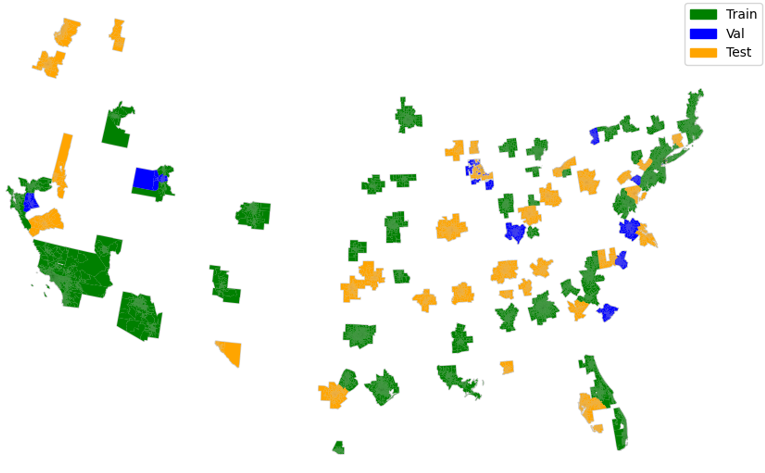
\includegraphics[width=\linewidth,height=4.2cm,keepaspectratio]{figures/image15.png}
\column{.42\textwidth}
\begin{itemize}
\item National test: held-out cities
\item Temporal validation: held-out acquisitions in training cities
\item NYC: held-out tracts and a different imagery source
\end{itemize}
\end{columns}
\par\vfill\small NYC is a tract/sensor test; it is not a wholly unseen-city claim.

\note{1:00. City partitions from supplied split map and manuscript. Separate buffered NYC/Chicago tract holdouts can exist within training cities. Avoid absolute no-spatial-leakage claim across every evaluation. Temporal heldout year is interpolation, not future forecasting. Full split and selection details in backup; source map is inherited, not regenerated.}
\end{frame}

\begin{frame}[label=s22]{Tract rankings transfer to held-out cities}
\begin{center}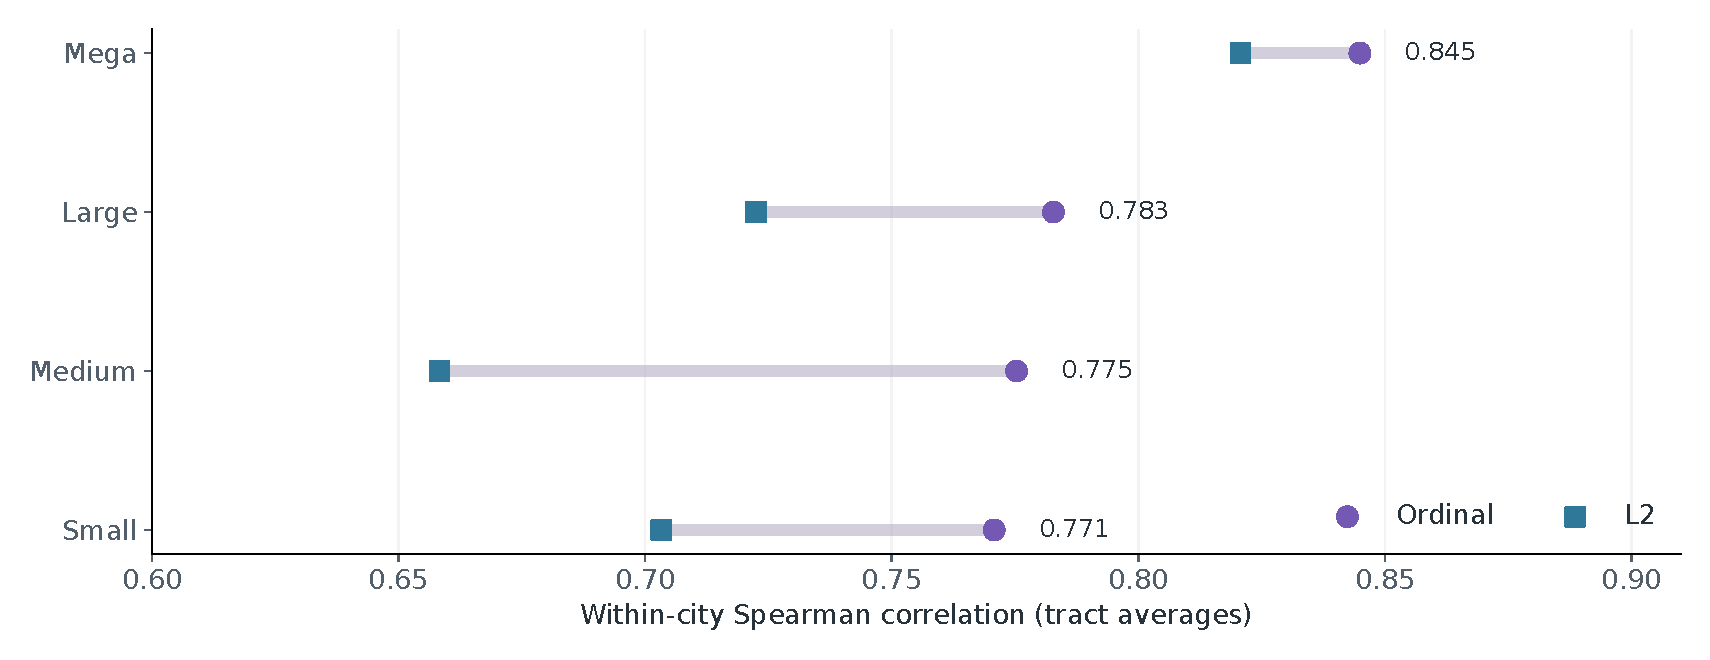
\includegraphics[width=\textwidth,height=0.53\textheight,keepaspectratio]{figures/revised/ranking_brackets.pdf}\end{center}
\takeaway{Paired test cells: Spearman 0.782 (ordinal) versus 0.711 (L2).}
\source{Tract averages; 158 matched city-year cells. Saved-run comparison; budgets differ.}

\note{1:00. Replotted from evaluation/US\_summary.json l2/bracket/rho and l2/all entries. This is matched-cell, tract-aggregate comparison. Do not mix with US\_A\_summary.csv building-level within Spearman .580 or pooled tract .727, which use different units/samples. L2 selected from 3 learning rates; full runs 750 vs 200 epochs.}
\end{frame}

\begin{frame}[label=s23]{The ordinal run improves rankings in 35 of 36 cities}
\begin{center}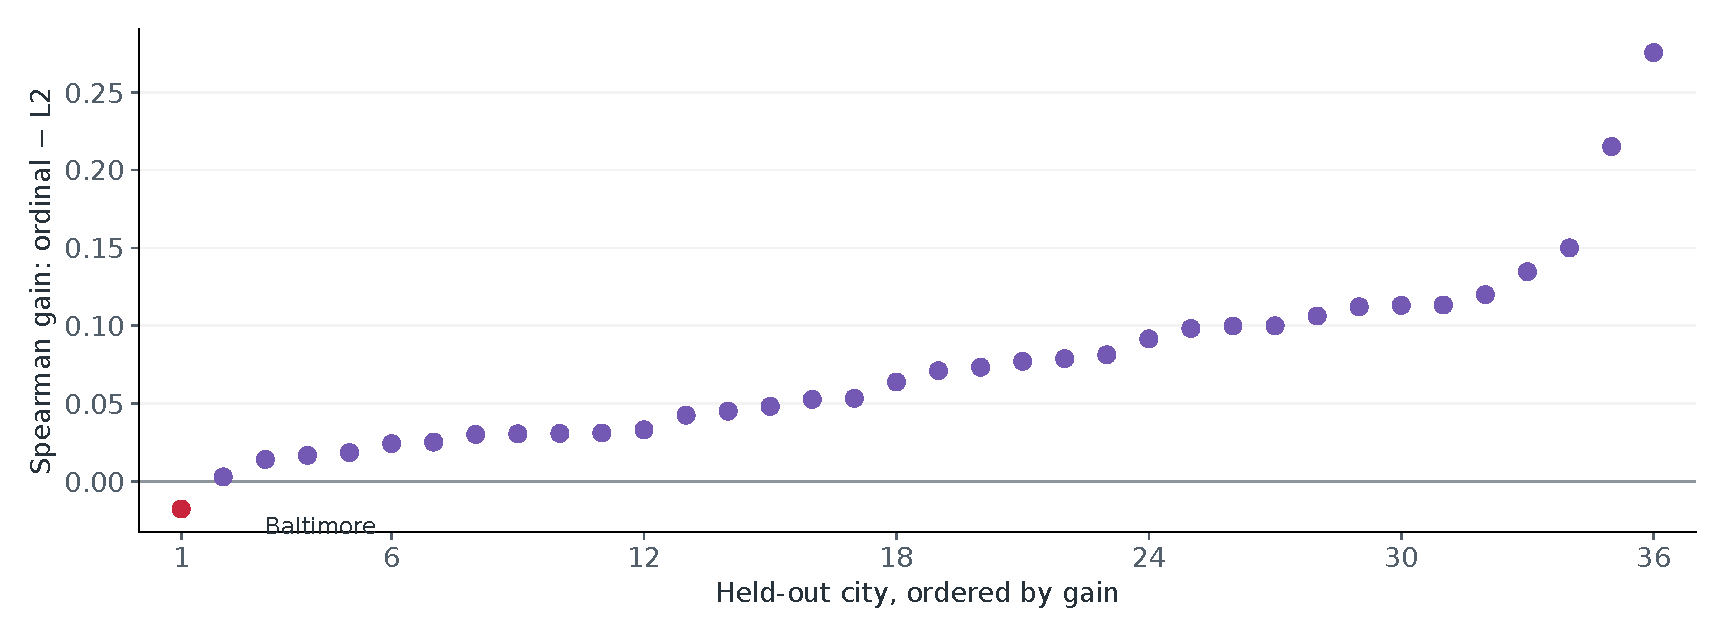
\includegraphics[width=\textwidth,height=0.53\textheight,keepaspectratio]{figures/revised/city_gains.pdf}\end{center}
\takeaway{Mean city gain: about 0.072 in within-city Spearman correlation.}
\source{One point per held-out city; negative gain in Baltimore. Training budgets differ.}

\note{0:45. Replotted without changes to data from US\_L2\_city\_distance.csv, sorted by difference. Broad advantage of these fitted runs. Do not infer causal effect of loss alone. Matched-budget selection diagnostics in backup show advantage remains at <=200 epochs, but are validation scores, not matched test-city results. Signed-distance slope includes zero; original figure retained in backup.}
\end{frame}

\begin{frame}[label=s24]{Persistence is high; detecting change is harder}

\begin{columns}[T]
\column{.45\textwidth}
\textcolor{mgAccent}{\textbf{Rank autocorrelation}}\par\bigskip
\begin{tabular}{@{}lr@{}}Predicted & \Large 0.936\\[.35cm]Label benchmark & \Large 0.931\end{tabular}
\column{.49\textwidth}
\textcolor{mgAccent}{\textbf{Changed versus stable groups}}\par\bigskip
Mean absolute score movement:\par\medskip
0.224 versus 0.220\par\medskip
Ratio: \textbf{1.02}; sign agreement: \textbf{50.1\%}
\end{columns}
\par\vfill\takeaway{A persistent score need not measure economic changes accurately.}
\source{US test set; groups defined by the survey-based change flag}

\note{1:00. Exact values from US\_B\_rank\_autocorr.csv. Autocorrelation summarizes stable-building pairs by city with pair-count weights; movement statistics use all available year pairs in each flag group. Mean absolute score displacement is in raw score units, not standardized change. Sign agreement is with label change in changed group (ties excluded). Different denominators; do not infer statistically significant separation from 1.02 ratio.}
\end{frame}

\begin{frame}[label=s25]{Construction tests responsiveness of the fitted index}

\begin{itemize}
\item Event: new footprint area crosses 1\%, 5\% or 10\% of baseline area
\item Control: tracts that never cross 1\%
\item Outcome: tract-average \textbf{predicted index}
\end{itemize}
\par\vspace{.3cm}
\[
\mathrm{ATT}_{\hat s}(q,t)
=\mathbb E[\bar{\hat s}_{it}(q)-\bar{\hat s}_{it}(\infty)\mid G_i=q]
\]
\par\vfill\takeaway{A response in the score is not a causal effect on true wealth.}

\note{1:00. q denotes construction cohort, avoiding conflict with head g. Callaway-SantAnna estimates on generated outcome require identification assumptions, including appropriate parallel trends and anticipation. Lipschitz bounds near pairs; does not imply direction for construction. Economic expectation of positive score change is a hypothesis, not a theorem. New construction is heterogeneous and need not always house wealthier residents.}
\end{frame}

\begin{frame}[label=s26]{NYC scores rise around construction}

\small Held-out tracts; anticipation = 2 periods $\approx$ 4 years
\begin{center}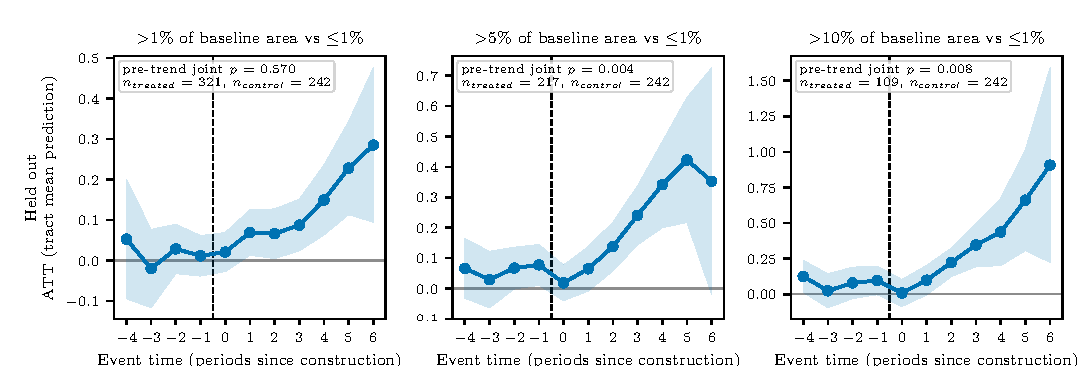
\includegraphics[width=\textwidth,height=0.52\textheight,keepaspectratio]{figures/revised/nyc_event_test.pdf}\end{center}
\par\vfill\takeaway{Joint pretrend tests: $p=.570$, $.004$, $.008$.}

\note{1:15. Top held-out row of the original plot, not a newly estimated event study. All three panels and confidence bands retained. First-threshold p=.570. Anticipation two means event adoption shifted two periods (~four years) early as in original title; labels refer to recorded construction. Do not claim clean causal dose response or robust identification. Full train/test figure and other cities in backup.}
\end{frame}

\begin{frame}[label=s27]{Fine spatial detail, with tract-level validation}
\begin{center}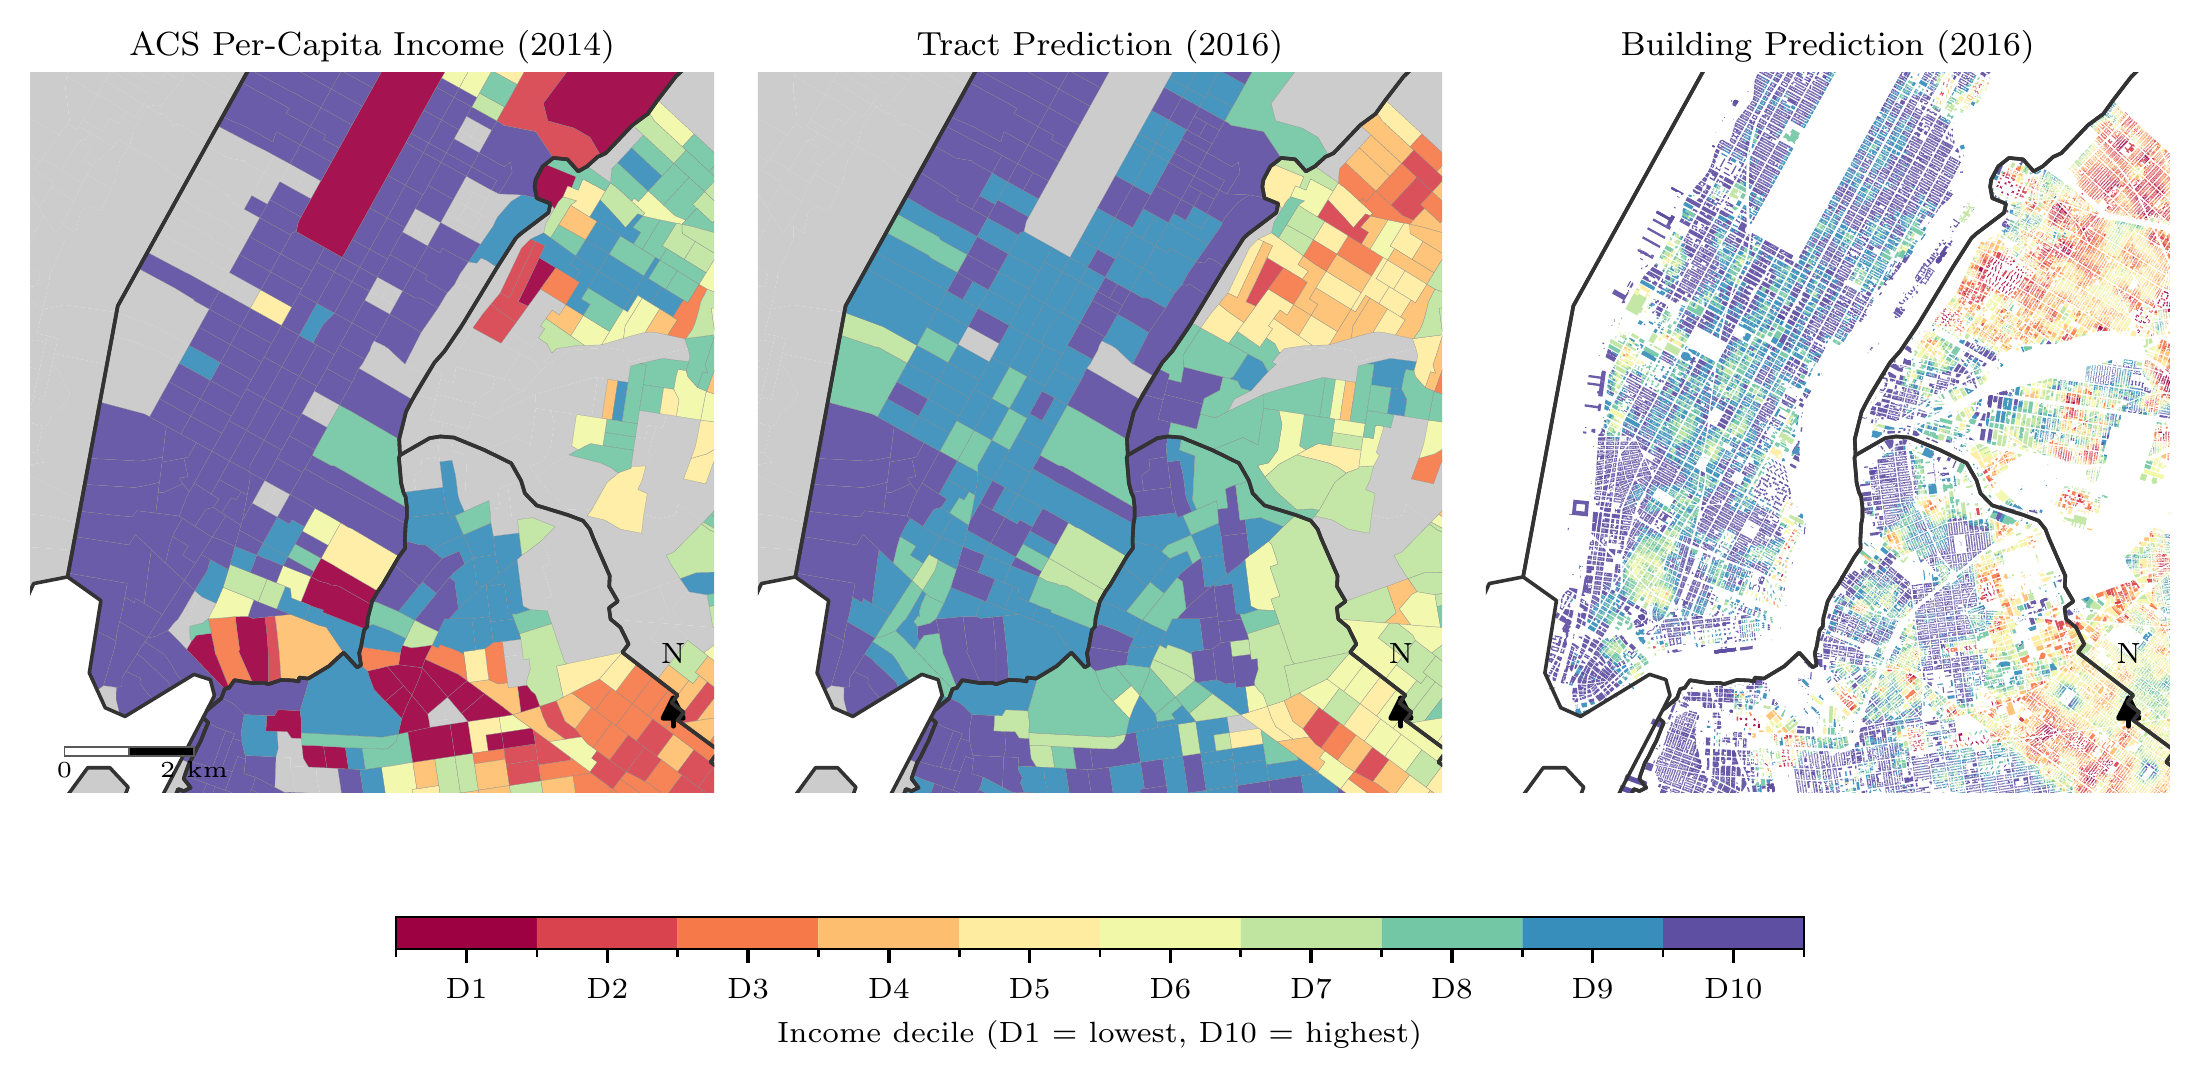
\includegraphics[width=\textwidth,height=0.64\textheight,keepaspectratio]{figures/revised/nyc_map.png}\end{center}
\source{2016 model predictions; 2014 ACS income benchmark. Spatial illustration.}

\note{0:45. Inspect original legend and dates. Inherited map compares ACS and model geography at different resolution. Use as a visual illustration, not proof of within-tract accuracy. Building scores inherit tract supervision, and local tiles contain surrounding neighborhood context.}
\end{frame}

\begin{frame}[label=s28]{Held-out tract changes remain poorly predicted}
\begin{center}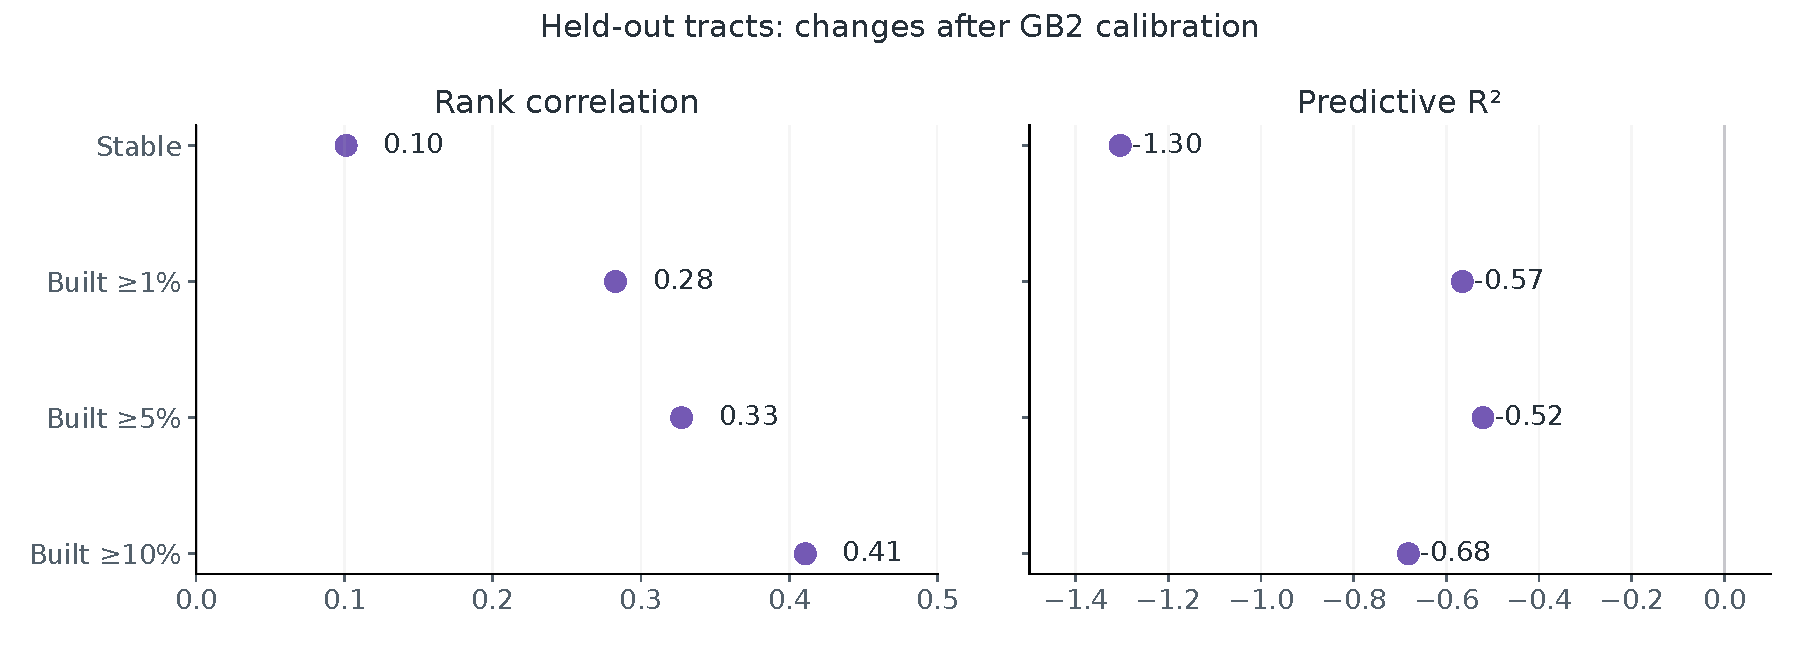
\includegraphics[width=\textwidth,height=0.53\textheight,keepaspectratio]{figures/revised/change_heldout.pdf}\end{center}
\takeaway{Predictive $R^2$ is negative in every construction group.}
\source{ACS 2013--2023; imagery 2010--2012 versus 2020--2022. Groups are nested.}

\note{1:45. Replotted from explicit heldout columns of F\_construction\_scatter.csv. Heldout n=243,371,196,86 for stable, >=1\%, >=5\%, >=10\%. Spearman .101,.283,.327,.411; predictive R2 -1.304,-.566,-.521,-.682. These are point estimates without uncertainty intervals. Full mixed-sample scatter retained in backup. Both sides use GB2 dollar mappings; not raw Delta f, and mapping uses target-year survey information. Negative predictive R2 indicates poor change-level calibration, even when rank correlation is positive.}
\end{frame}

\begin{frame}[label=s29]{Temporal measurement requires more than stable images}

\[
\Delta R_i=\Delta f(X_i)+\Delta\varepsilon_i
\]
\[
\Delta W_i=\psi_{c,t'}(R_{i,t'})-\psi_{ct}(R_{it})
\]
\begin{itemize}
\item Occupant changes and survey noise can move $R$ without visible construction
\item The measurement map $\psi_{ct}$ can change even if $R$ does not
\item Calibrating each date to a survey is not a test of unseen-date dollar prediction
\end{itemize}

\note{1:00. Corrects original assertion that all label change at stable places is epsilon. That ignores psi changes. Do not claim most tracts meet A3 or delta f=0 by design. Noise-ceiling calculation needs covariance across ACS releases, generated-index uncertainty and measurement-error assumptions; a simple formula is not an empirical ceiling for Delta f.}
\end{frame}

\begin{frame}[label=s30]{What is established, and what comes next}

\textcolor{mgAccent}{\textbf{Established so far}}\par\medskip
A framework for within-cell recovery; strong US tract rankings;\par
construction responsiveness with identification caveats.
\par\vspace{.6cm}
\textcolor{mgAccent}{\textbf{Questions for this lab}}\par\medskip
\begin{enumerate}
\item What restrictions align cities without imposing false stability?
\item What data would validate genuine economic changes?
\item When can an effect on the score recover an effect on wealth?
\end{enumerate}

\note{1:15. End on the substantive result and three research decisions. Monte Carlo evidence should be incorporated verbally after actual figures arrive. Near-term work: label-independent pair selection, ratio penalty, heteroskedastic comparison models, held-out change validation, calibration, inference for target functional. Inference cannot be dismissed because neural weights are nonidentified; downstream design determines dependence and resampling. Leave this slide up for discussion rather than a separate thank-you.}
\end{frame}
\appendix
\begin{frame}[label=errors]{A4: three comparison-error models}

\begin{tabularx}{\textwidth}{@{}l X@{}}
Median zero + strict crossing & $p_{ij}>1/2\iff\Delta_{ij}f>0$\\[.6cm]
Cell-specific logistic & $p_{ij}=\Lambda(\rho_{ct}\Delta_{ij}f)$\\[.6cm]
Common logistic & $p_{ij}=\Lambda(\rho\Delta_{ij}f)$
\end{tabularx}
\par\vfill\small Current theoretical results use the third case.\hfill\hyperlink{s12}{\beamerreturnbutton{Back}}

\note{Median zero requires the appropriate strict crossing/no-flat-region condition for the equivalence, not simply a loose median definition. Homogeneous logistic errors refer to residual differences.}
\end{frame}

\begin{frame}[label=sampling]{A5--A6: sampling and estimation}
\begin{itemize}
\item Independent, identically distributed cities; arbitrary within-city dependence
\item Bounded city and pair counts; positive expected counts; fixed $T$
\item Compact $\Theta$, continuous scores in parameters, uniformly bounded scores
\item $\inf_\Theta Q<\log2$; optimization error $\eta_C\to_p0$
\end{itemize}\par\vfill\hyperlink{s15}{\beamerreturnbutton{Back}}
\note{The near-minimizer condition is an assumption about optimization, not a guarantee from adding more cities.}
\end{frame}

\begin{frame}[label=proof]{Theorem 1: why the population bound holds}

\textbf{1. Ranking loss is minimized at $\rho f$.}
\[
Q_{\rm cross}(s)\ge Q_{\rm cross}(\rho f)
\]
\textbf{2. The true index pays little stability penalty.}
\[
S(f)\le L^2\delta^2,\quad V(f)=1
\]
\textbf{3. Logistic curvature bounds errors in differences.}
\[
Q_{\rm cross}(s)-Q_{\rm cross}(\rho f)
\ge\tfrac12\Lambda'(B)\mathbb E_{\mathcal C}[\Delta_{ij}(s-\rho f)^2]
\]
\hfill\hyperlink{s14}{\beamerreturnbutton{Back}}

\note{Second-order expansion is for conditional expected pairwise loss with true p; integrate over pair distribution. B must bound both differences along segment.}
\end{frame}

\begin{frame}[label=b4]{Pooling levels estimates a mixture}

Under the latent model, the general identity is
\[
\mathbb E[W\mid X=x]=\sum_{c,t}\Pr(c,t\mid X=x)
\mathbb E[\psi_{ct}(f(x)+\varepsilon)\mid X=x,c,t].
\]
\medskip
Under the separate additive-outcome model\par
$W=\psi_{ct}(f(X))+u$, with $\mathbb E[u\mid X,c,t]=0$:
\[
\mathbb E[W\mid X=x]=\sum_{c,t}\Pr(c,t\mid X=x)\psi_{ct}(f(x)).
\]
\par\vfill\small The shorter formula does not follow from latent mean-zero errors alone.

\note{}
\end{frame}

\begin{frame}[label=b5]{Label construction and interpretation}

\begin{itemize}
\item Earnings and capital income are expressed per resident
\item Human wealth uses an ordinary finite annuity with tract-specific horizon
\item Housing equity uses $(A^H/P)(1-m\ell_t)$ in the code
\item $\ell_t$ is derived from aggregate Federal Reserve equity shares
\end{itemize}
\par\vfill\takeaway{The economic interpretation of aggregate LTV and mortgage-share scaling needs scrutiny.}

\note{This is a source-code audit, not a change to label data. An aggregate owners-equity ratio is not necessarily a conditional mortgaged-owner LTV, so using both factors deserves conceptual checking. Missing component fallbacks also affect interpretation. No underlying model/data edits were made.}
\end{frame}

\begin{frame}[label=b6]{Training details from the saved run}

\begin{tabularx}{\textwidth}{@{}l X@{}}
Backbone & ScaleMAE; local imagery score network\\[.3cm]
Input & 224 pixels; 112m radius; 10m centroid jitter\\[.3cm]
Optimization & Learning rate $10^{-4}$; 750 epochs; batch size 8\\[.3cm]
Loss weights & $\lambda_s=0.3$, $\lambda_{\rm var}=1.5$\\[.3cm]
Temporal share & 0.4; tract sampling enabled\\[.3cm]
Selection & Saved setting: within\_50\_50
\end{tabularx}

\note{Source models/run\_20260722/run\_20260722\_logs.txt. Architectural LoRA specifics in older prose were not re-verified from a saved checkpoint, so omitted here. Effective batch details should be confirmed if discussed.}
\end{frame}

\begin{frame}[label=b7]{Current pair gate uses survey outcomes}

\[
Z_{it}=\frac{\log W_{it}-\mu_{ct}}{\sigma_{ct}},\qquad
S_i=\frac{|Z_{i,2023}-Z_{i,2014}|}{\sqrt{\widetilde{SE}_{2023}^2+\widetilde{SE}_{2014}^2}}
\]
\begin{itemize}
\item Current rule treats a non-rejection at 10\% as stable
\item This is not label-independent pair selection
\item Failure to reject does not establish physical or economic stability
\end{itemize}
\par\vfill\small Proposed alternative: independently selected footprint or image-change pairs.

\note{W2 uses replicate-based component covariance in current process\_acs. Do not use a generic independent-component delta method for the entire index. Exact vintages in saved pair table should be confirmed before claims about the run gate.}
\end{frame}

\begin{frame}[label=b8]{Comparison at a common training budget}

\begin{tabular}{@{}lrr@{}}
\toprule
Run & Budget & Best selection score\\\midrule
Ordinal & $\le200$ epochs & 0.606\\
L2 & $\le200$ epochs & 0.535\\
Ordinal & 750 epochs & 0.641\\\bottomrule
\end{tabular}
\par\vspace{.6cm}
\takeaway{These are validation-selection scores, not matched-budget test results.}
\source{US\_L2\_matched\_budget.csv; L2 learning rate selected from three candidates}

\note{At <=200, ordinal best epoch197; L2 best98. Full ordinal best708. Do not label these Spearman on the same test cities: selection is a combined validation metric. This qualifies only-loss-differs claims.}
\end{frame}

\begin{frame}[label=b9]{Training curves}
\begin{center}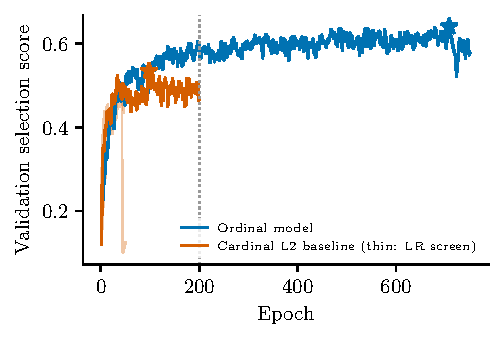
\includegraphics[width=\textwidth,height=0.70\textheight,keepaspectratio]{figures/revised/training.pdf}\end{center}
\note{}
\end{frame}

\begin{frame}[label=b10]{Ranking gains versus distance from training cities}
\begin{center}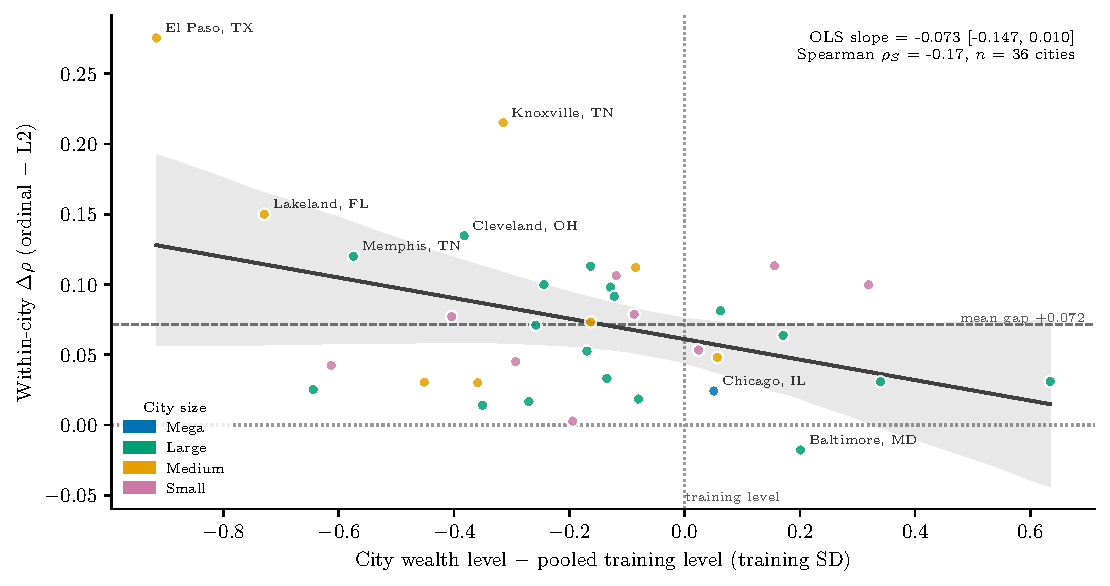
\includegraphics[width=\textwidth,height=0.60\textheight,keepaspectratio]{figures/revised/gap_distance.pdf}\end{center}\small Slope interval includes zero; distance gradient is suggestive.
\note{}
\end{frame}

\begin{frame}[label=b11]{Full national performance figure}
\begin{center}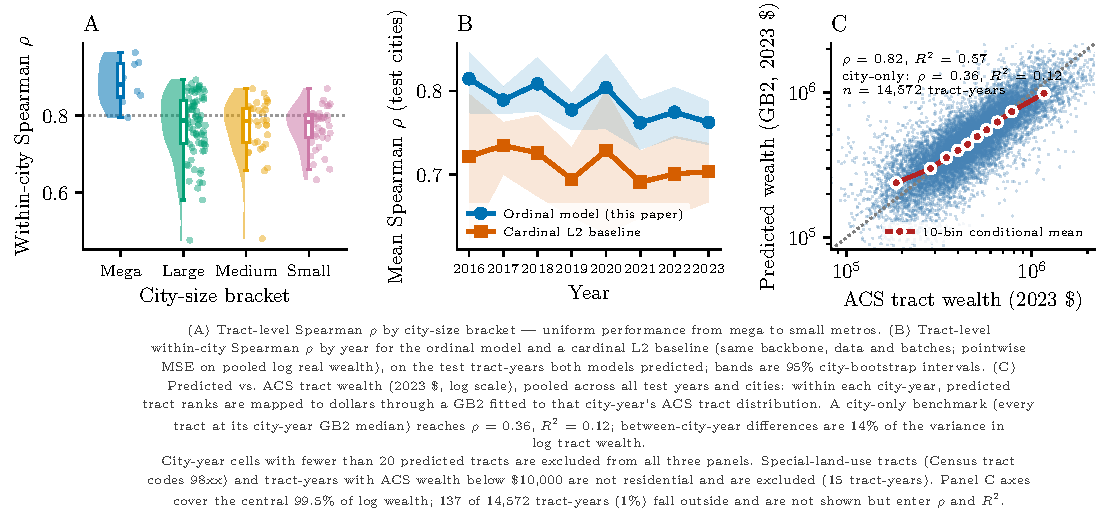
\includegraphics[width=\textwidth,height=0.56\textheight,keepaspectratio]{figures/revised/us_performance.pdf}\end{center}\small Distinguish within-city ranking from pooled and calibrated-dollar performance.
\note{}
\end{frame}

\begin{frame}[label=b12]{NYC construction event study: all reported panels}
\begin{center}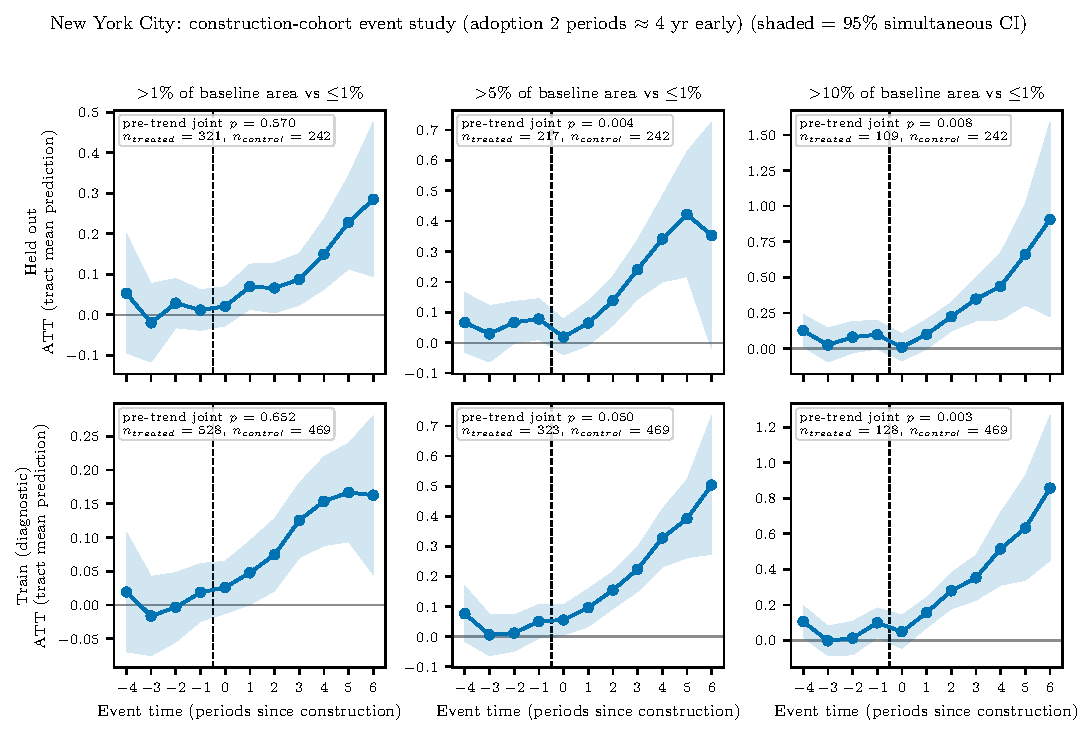
\includegraphics[width=\textwidth,height=0.70\textheight,keepaspectratio]{figures/revised/nyc_event_full.pdf}\end{center}
\note{Top = held-out; bottom = training. Retain pretrend tests and simultaneous intervals. Higher thresholds have smaller samples and different treated compositions; not a causal dose-response comparison.}
\end{frame}

\begin{frame}[label=b13]{NYC change prediction: all construction groups}
\begin{center}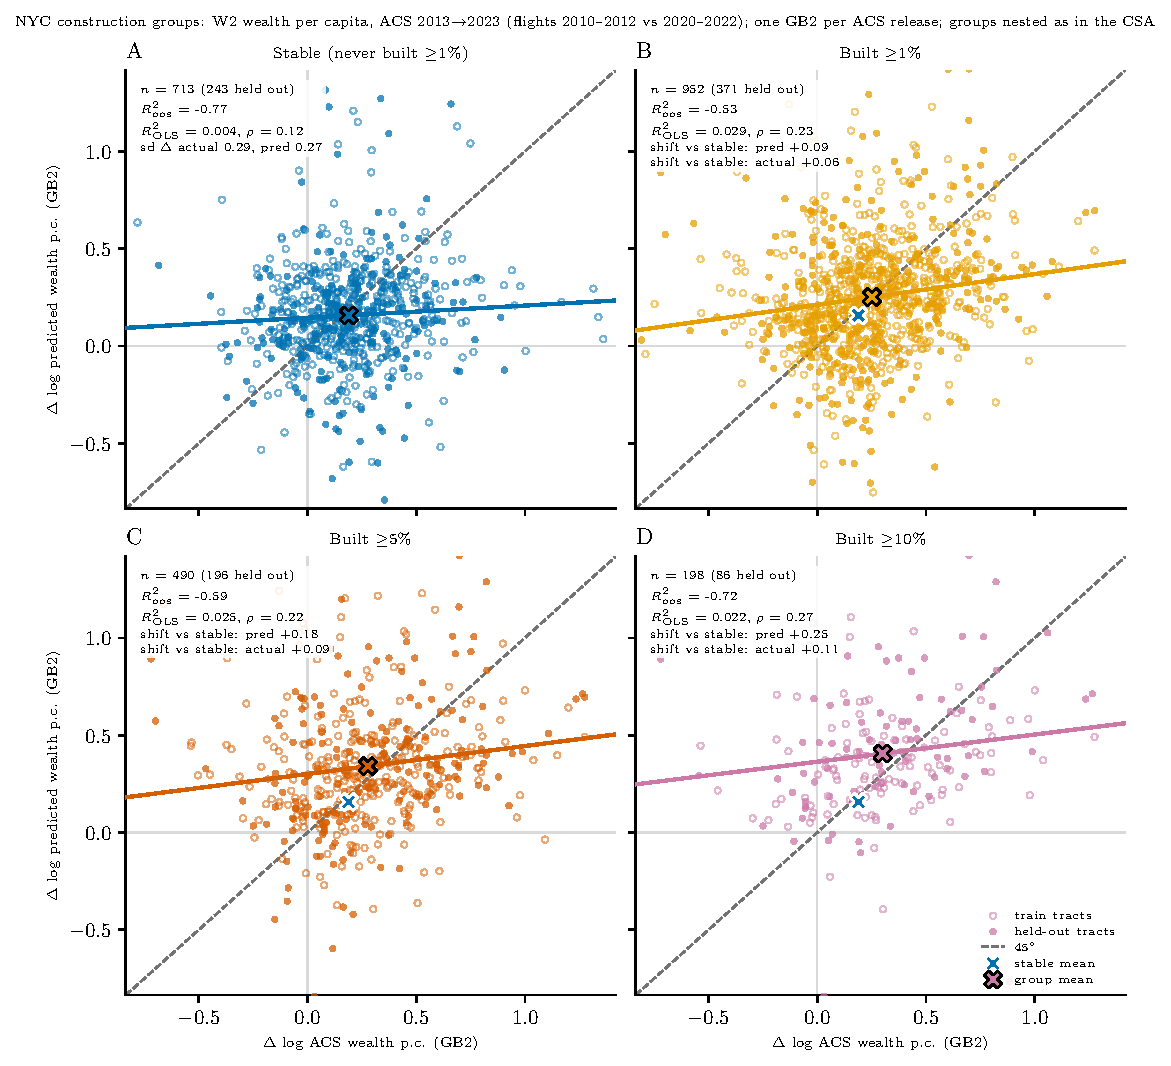
\includegraphics[width=\textwidth,height=0.70\textheight,keepaspectratio]{figures/revised/nyc_change_full.pdf}\end{center}
\note{Open training and filled held-out points; displayed fit statistics aggregate available plotted sample. GB2 mapping uses each target release. This is not raw delta f.}
\end{frame}

\begin{frame}[label=b14]{Tampa: construction event study}
\begin{center}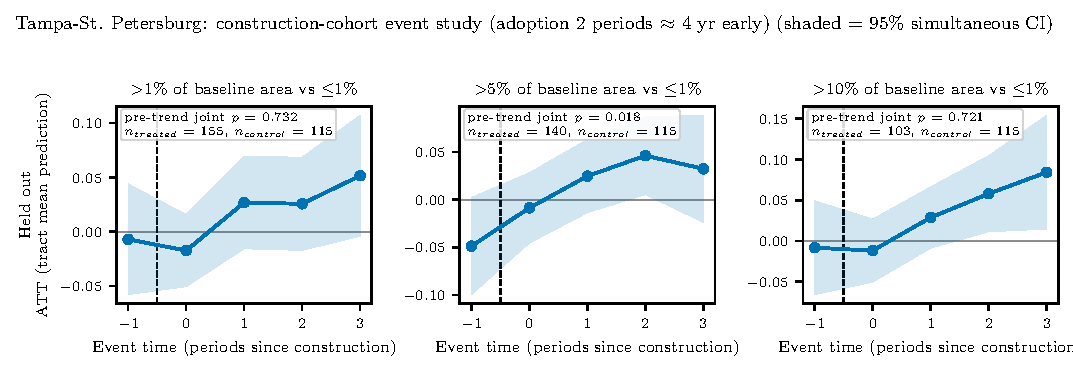
\includegraphics[width=\textwidth,height=0.73\textheight,keepaspectratio]{figures/revised/tampa.pdf}\end{center}
\note{}
\end{frame}

\begin{frame}[label=b15]{Seattle: construction event study}
\begin{center}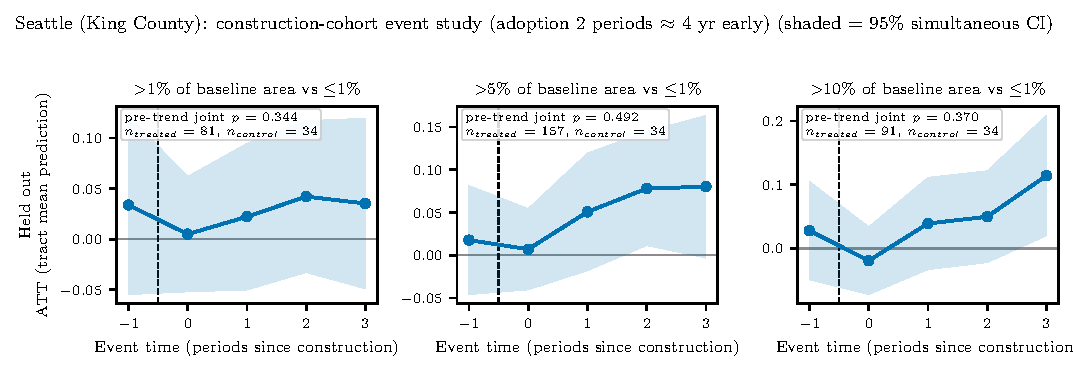
\includegraphics[width=\textwidth,height=0.73\textheight,keepaspectratio]{figures/revised/seattle.pdf}\end{center}
\note{}
\end{frame}

\begin{frame}[label=b16]{NYC: income benchmark and predicted deciles}
\begin{center}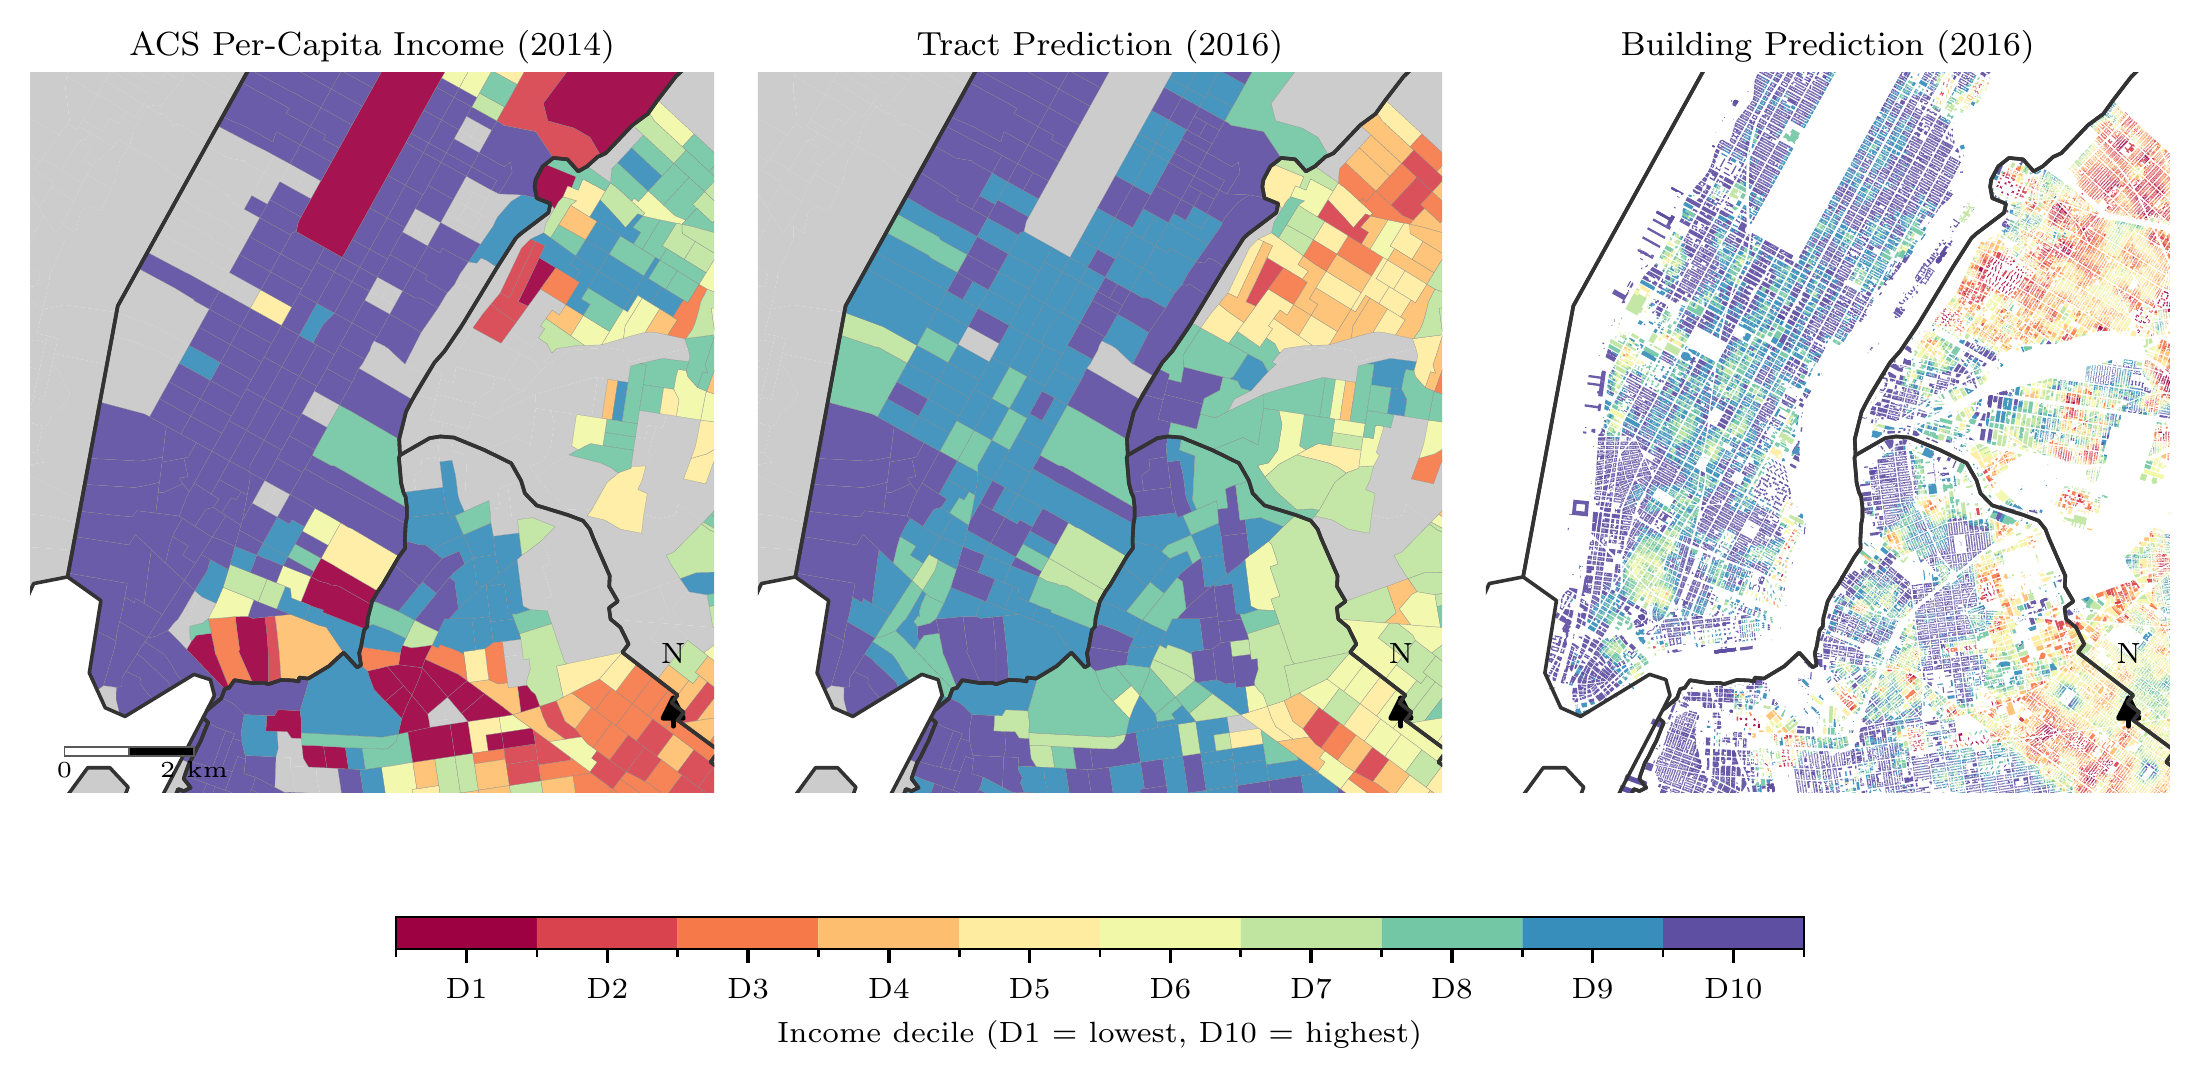
\includegraphics[width=\textwidth,height=0.70\textheight,keepaspectratio]{figures/revised/nyc_map.png}\end{center}
\note{}
\end{frame}

\begin{frame}[label=b17]{Testing sensitivity to imperfect stable pairs}
\begin{itemize}
\item Exact links: hold signal fixed and redraw acquisition noise
\item Drift: allow a bounded change in the latent index
\item False links: join unrelated units, randomly or asymmetrically
\item Compare fixed versus validation-selected $\lambda$
\end{itemize}
\note{Proposed MC4 design. No results are claimed; add actual figures when available.}
\end{frame}

\begin{frame}[label=b18]{Inference and downstream evaluation}
\begin{itemize}
\item Uncertainty enters through surveys, fitted scores, calibration and the research design
\item Nonidentification of network weights does not rule out inference on functionals
\item Training-city clustering and evaluation-design clustering are different questions
\item Predicted-outcome effects require assumptions or correction for differential prediction error
\end{itemize}
\note{Conformal coverage and prediction-powered inference are not automatic solutions for dependent spatial panels or causal outcomes. Need setting-specific assumptions, labeled validation, and target functional. No generic independence of treatment and prediction error sufficient for every design.}
\end{frame}

\begin{frame}[label=b19]{References used in the talk}

\small
\begin{itemize}
\item Aiken et al. (2022), \emph{Nature}: targeting humanitarian aid
\item Jean et al. (2016), \emph{Science}; Yeh et al. (2020), \emph{Nature Communications}: poverty from imagery
\item Khachiyan et al. (2022), \emph{AER: Insights}: microspatial economic growth
\item Zheng et al. (2026), arXiv:2604.23166: Tempov
\item Burges et al. (2005), ICML: RankNet
\item Callaway and Sant'Anna (2021), \emph{Journal of Econometrics}: staggered DiD
\end{itemize}

\note{}
\end{frame}
\end{document}
